%En esta sección se \textcolor{red}{Agregar Texto}
%
%\begin{figure}[ht]
%    \centering
%    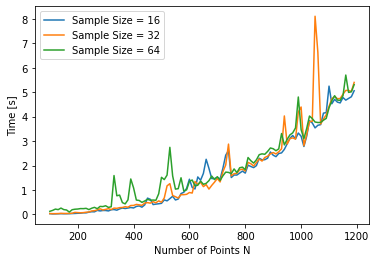
\includegraphics[width=8cm]{img/tesis/resultados/dpp_sample_time.%png}
%    \caption{Tiempo de Sampleo DPP según cantidad de datos}
%    \label{fig:dpp_sampling_time}
%\end{figure}

\section{Muestreo Clase Minoritaria}

Los procesos puntuales determinantales permiten muestrear subconjuntos de datos de tal forma que exista una alta repulsión entre sus elementos. Esta repulsión depende de una métrica de distancia que es complicada de construir en datos con dimensiones altas y que puede variar según la tipología del dato. 

\begin{images}[\label{fig:sampling}]{\centering Comparación de un muestreo de tamaño 32 sobre el dataset de clasificación binaria en 2 dimensiones utilizando una estrategia uniforme y una con DPP.}
    \addimage{img/tesis/resultados/sampling_uniforme.png}{width=5cm}{Sampling Uniforme}
    \addimage{img/tesis/resultados/sampling_DPP.png}{width=5cm}{Sampling DPP}

\end{images}

Cuando se trabaja en un dataset de 2 dimensiones, la metrica euclidiana rescata perfectamente la distancia entre pares de ejemplos. La primera parte del experimento tiene como objetivo mostrar la diferencia entre un sampling uniforme y un sampling mediante un DPP en 2 dimensiones. Como se puede ver en la Figura \ref{fig:sampling} (a), un método uniforme samplea en función del desbalance del dataset $\frac{C_0}{C_1} = 1/2$, en este caso 13 elementos de la clase 0 y 19 de la clase 1. Por otro lado, al samplear mediante un DPP en Figura \ref{fig:sampling} (b), se asigna una menor probabilidad a muestrear puntos que se encuentren espacialmente cercanos, por lo que no se espera una alta densidad en $C_1$ como en el caso uniforme. El experimento efectivamente comprueba este resultado, pues se obtienen 16 puntos para la clase 0 y 16 puntos en la clase 1.

\vspace{0.2cm}

\begin{figure}[ht]
    \centering
    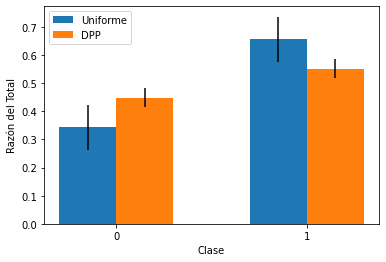
\includegraphics[width=8cm]{img/tesis/resultados/sampling_n_2.png}
    \caption{Razón del total promedio ($n=100$) de ejemplos sampleados en el dataset de 2 dimensiones. Las barras azules representan las proporciones para un sampling uniforme y las barras naranjas para el sampling con DPP, las barras negras verticales corresponden a la varianza de los datos.}
    \label{fig:proporcion_sampling}
\end{figure}

Iterando el ejercicio una mayor cantidad de veces ($n=100$) y promediando sus resultados se obtiene Figura \ref{fig:proporcion_sampling}. Como se puede ver en esta figura, el método uniforme en promedio samplea en función del desbalance del dataset (barras azules) y con una alta varianza. En cambio, el sampleo con un DPP (barras naranjas) muestrea de manera más homogénea, cercano a la proporción 1:1 entre clases y con una menor varianza. 

\vspace{0.2cm}

Lo anterior permite concluir que la metodología de sampleo con un DPP permite crear consistentemente \textit{batches} con áreas de menor densidad de puntos y mayor presencia de elementos de las clases minoritarias. 

\vspace{0.2cm}

En esta segunda parte del primer experimento, se repite el mismo ejercicio con el dataset \textit{Fashion MNIST} pero ahora comparando las distintas métricas de distancia (que utiliza el DPP) presentadas en la metodología. Con el fin de disminuir el costo de muestreo, se considera el siguiente conjunto reducido de ejemplos (Tabla \ref{table:fashion_mnist_val}) pero que sigue la misma distribución que el presentado en la Tabla \ref{table:fashion_mnist}.

\begin{table}[ht]
\begin{tabular}{|c|c|c|c|c|c|c|c|c|c|c|}
\hline
Clase    & 0    & 1    & 2    & 3    & 4    & 5    & 6   & 7   & 8   & 9   \\ \hline
Cantidad & 250 & 250 & 250 & 250 & 150 & 150 & 150 & 50 & 50 & 50 \\ \hline
(\%) & 15.62 & 15.62 & 15.62 & 15.62 & 9.37 & 9.37 & 9.37 & 3.13 & 3.13 & 3.13 \\ \hline
\end{tabular}
\caption{Validación - Clasificación Multiclase. Total = 1600.}
\label{table:fashion_mnist_val}
\end{table}

Para el aprendizaje de la métrica de distancia basados en el \textit{Autoencoder} o en la red \textit{Oneshot}, se mantuvo la arquitectura presentada en la sección anterior pero cambiando el tamaño del espacio latente a uno de largo 16 y se entrenan con el mismo conjunto de entrenamiento (Tabla \ref{table:fashion_mnist}). Con el único fin de visualizar las representaciones, se aplicó una técnica de reducción de dimensionalidad \textit{UMAP} \cite{https://doi.org/10.48550/arxiv.1802.03426}

\begin{images}[\label{fig:umap_representation}]{\centering Visualización en 2 dimensiones de Fashion-MNIST mediante la técnica de reducción dimensionalidad UMAP utilizada sobre la representación latente entregada por el \textit{Autoencoder} y la red \textit{Oneshot} luego de ser entrenados.}
    \addimage{img/tesis/resultados/oneshot_umap.png}{width=7cm}{Representación Oneshot}
    \addimage{img/tesis/resultados/autoencoder_umap.png}{width=7cm}{Representación Autoencoder}

\end{images}

Como se aprecia en Figura \ref{fig:umap_representation} la técnica UMAP calculada sobre la representación entregada por la red \textit{Oneshot} (a) y  \textit{Autoencoder} (b) permite verificar que las clases se encuentran correctamente separadas (diferencias entre-clases, visualmente mejor en (a)) y que por sobre todo, existen ``clusters'' dentro de una misma clase (diferencias intra-clase) que el DPP permitiría representar. No se utilizará esta representación \textit{UMAP} para los experimentos pero está dentro de los trabajos a realizar en el futuro. 

\begin{figure}[ht]
    \centering
    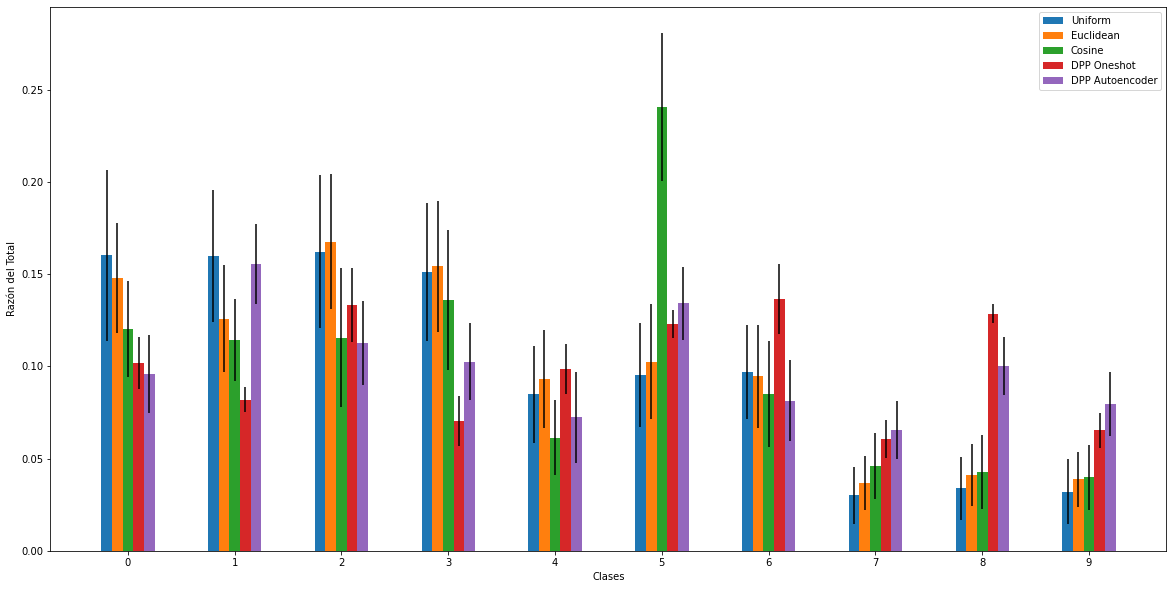
\includegraphics[width=12cm]{img/tesis/resultados/sampling_n_10.png}
    \caption{Razón del total promedio ($n=50$) de ejemplos muestreados en el dataset Fashion-MNIST. La barra azul corresponde a un sampleo uniforme y el resto de barras corresponden a distintas métricas utilizadas para el sampleo con un DPP.}
    \label{fig:proporcion_sampling_mnist}
\end{figure}

La Figura \ref{fig:proporcion_sampling_mnist} corresponde a la proporción de ejemplos sampleados en $n=50$ iteraciones entre las distintas clases y para cada una de las métricas propuestas. Notar que la métrica euclidiana junto a un kernel RBF (barra naranja) tiene un comportamiento similar al de un sampleo uniforme (barra azul) pues se ve afectada por la maldición de la dimensionalidad, es decir, la métrica euclidiana no permite diferenciar clases debido a la alta dimensión de los vectores. Por otro lado, si bien la magnitud de los vectores no afecta a la distancia coseno (barra verde) y debiese ser más robusta a la dimensión, esta tampoco muestra un comportamiento considerablemente distinto al de los 2 anteriores. 

\vspace{0.2cm}

Ahora bien, la distancia euclidana aplicada sobre una representación de baja dimensionalidad (\textit{Oneshot} y \textit{Autoencoder}, barra roja y morada respectivamente) si muestran un comportamiento considerablemente distinto pues samplean con mayor frecuencia las clases minoritarias 7, 8 y 9.

\begin{figure}[ht]
    \centering
    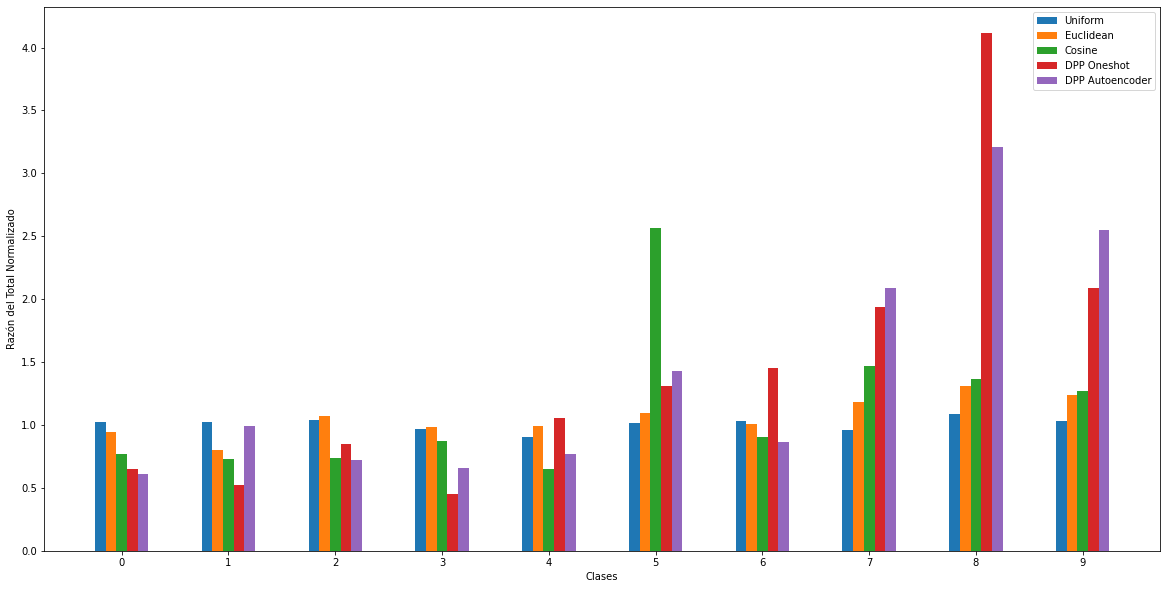
\includegraphics[width=12cm]{img/tesis/resultados/sampling_n_10_normalizado.png}
    \caption{Razón del total normalizada promedio (n = 50) de ejemplos muestreados en el dataset Fashion-MNIST. La normalización se realizó en función del desbalance del dataset.}
    \label{fig:normalizado_sampling_mnist}
\end{figure}

\vspace{0.2cm}

Normalizando por la proporción de ejemplos en cada clase con respecto al total, se obtiene la Figura \ref{fig:normalizado_sampling_mnist}. Un comportamiento uniforme debería reflejarse como un valor 1 en la gráfica (samplear en función del desbalance del dataset). Notar que los métodos \textit{Oneshot} y \textit{Autoencoder} samplean de 3 a 4 veces más de lo esperado a las clases minoritarias y con una menor varianza, un comportamiento muy similar a lo que ocurría en el caso binario. 

\vspace{0.2cm}

Con lo anterior y dado que nuestro objetivo es utilizar un DPP centrado en una métrica que distinga las clases y samplee con mayor probabilidad a las clase minoritarias, se valida el uso de \textit{Oneshot} y \textit{Autoencoder} como las métricas que se usarán en las siguientes secciones. Se propone como trabajo futuro la búsqueda de métricas que no dependan del entrenamiento de un red para realizar esta tarea y que tengan efectos similares a los presentados (por ejemplo, la distancia fraccional).  

\section{Fast DPP}

El algoritmo propuesto en Algoritmo \ref{alg:alg4} se fundamenta en las primeras iteraciones del entrenamiento de una red neuronal. Para problemas de clasificación de baja dimensionalidad y una cantidad acotada de clases, la región de decisión se logra aproximar en unas cuantas iteraciones, mientras que para otros problemas más complejos, esto ocurrirá después. 

\begin{images}[\label{fig:baseline_it_n}]{\centering Primeras iteraciones SGD en el problema de clasificación binaria. Las zonas de color celeste y anaranjado delimitan la región de decisión del problema.}
    \addimage{img/tesis/resultados/baseline_it_1.png}{width=4cm}{Iteración 1}
    \addimage{img/tesis/resultados/baseline_it_2.png}{width=4cm}{Iteración 2}
    \addimage{img/tesis/resultados/baseline_it_3.png}{width=4cm}{Iteración 3}

\end{images}

\begin{images}[\label{fig:dpp_it_n}]{\centering Primeras iteraciones Fast DPP en el problema de clasificación binaria. Las zonas de color celeste y anaranjado delimitan la región de decisión del problema.}
    \addimage{img/tesis/resultados/dpp_it_1.png}{width=4cm}{Iteración 1}
    \addimage{img/tesis/resultados/dpp_it_2.png}{width=4cm}{Iteración 2}
    \addimage{img/tesis/resultados/dpp_it_3.png}{width=4cm}{Iteración 3}

\end{images}


Las Figuras \ref{fig:baseline_it_n} y \ref{fig:dpp_it_n} muestran las primeras 3 iteraciones del entrenamiento de una red neuronal que resuelve el problema de clasificación binaria en 2 dimensiones. Al igual que en la sección anterior, es posible notar que la selección de un \textit{batch} mediante el uso de un DPP (Figura \ref{fig:dpp_it_n}) tiene una mayor proporción de la clase minoritaria en comparación a la selección uniforme (Figura \ref{fig:baseline_it_n}). En consecuencia, la región de decisión luego de 3 iteraciones es mejor en Figura \ref{fig:dpp_it_n} (c) pues clasifica correctamente más ejemplos de la clase minoritaria (clase 0) y mantiene los correctamente clasificados de la clase mayoritaria (clase 1). 

\begin{images}[\label{fig:ambas_it_n}]{\centering Última iteración de las metodologías SGD y DPP si no se descartan ejemplos como lo propone Fast DPP.}
    \addimage{img/tesis/resultados/baseline_it_n.png}{width=6cm}{Última iteración SGD}
    \addimage{img/tesis/resultados/dpp_it_n.png}{width=6cm}{Última iteración DPP}

\end{images}

Si no descartamos ejemplos como lo propone \textit{Fast DPP}, es decir, descartar únicamente los ejemplos muestreados en cada \textit{mini batch} y no los $M$ que se proponen, las últimas iteraciones del algoritmo serían como lo muestra la Figura \ref{fig:ambas_it_n} (b) pues el conjunto del cual samplear es reducido y los ejemplos de la clase minoritaria ya fueron muestreados en su totalidad. Por otro lado, los rendimientos de ambos modelos (a) y (b) son bastante parecidos pues ambos observarían todos los ejemplos del dataset y no habría mayor diferencia (salvo en el tiempo de entrenamiento). 

\vspace{0.2cm}

Lo anterior justifica la utilización del algoritmo \textit{Fast DPP} que hace uso de la capacidad del DPP para samplear ejemplos diversos durante las primeras iteraciones de cada época (alcanzando así una ``buena'' región de decisión) sin la necesidad de mirar el resto de ejemplos, acelerando así el entrenamiento. 

\begin{images}[\label{fig:2d_fast_dpp}]{\centering Resultados Fast DPP en dataset clasificación binaria (30 iteraciones), M = 100.}
    \addimage{img/tesis/resultados/loss_2d_fast.jpg}{width=7cm}{Train loss según época}
    \addimage{img/tesis/resultados/val_loss_2d_fast.jpg}{width=7cm}{Val loss según época}
    \addimage{img/tesis/resultados/2d_fast_time.jpg}{width=7cm}{Val loss según tiempo}

\end{images}

Con respecto al entrenamiento en 10 épocas con un tamaño de sampling inicial $M = 100$ (es decir, descartando $M-k = 100-64 = 36$ ejemplos en cada iteración con $k$ el tamaño del \textit{batch}), según la Figura \ref{fig:2d_fast_dpp} (a) y (b), es claro que el método \textit{baseline} es superior durante todo el entrenamiento al método \textit{Fast DPP} según la métrica de \textit{loss}. Lo anterior es un resultado esperable de un algoritmo que no mira todos los ejemplos pues su función es la de acelerar el entrenamiento, lamentablemente, esto tampoco es logrado como lo muestra (c) pues la arquitectura de la red es poco profunda y los datos con los que trabaja de baja dimensionalidad (y en consecuencia, de bajo coste de procesamiento), por lo que el costo base de utilizar un DPP es superior a la de usar todos los datos para el entrenamiento.  

\vspace{0.2cm}

Cuando esto es aplicado sobre un conjunto de mayor complejidad como \textit{Fashion MNIST} donde el costo por iteración es más elevado (por la profundidad de la red y la dimensión de los datos), es cuando se puede apreciar la intención detrás de \textit{Fast DPP}.

\begin{images}[\label{fig:nd_fast_dpp}]{\centering Resultados Fast DPP en dataset clasificación multiclase (5 iteraciones), M = 400.}
    \addimage{img/tesis/resultados/loss_nd_fast.jpg}{width=7cm}{Train loss según época}
    \addimage{img/tesis/resultados/val_loss_nd_fast.jpg}{width=7cm}{Val loss según época}
    \addimage{img/tesis/resultados/time_nd_fast.jpg}{width=7cm}{Val loss según tiempo}

\end{images}

Como se puede notar en Figura \ref{fig:nd_fast_dpp} (a) y (b), el \textit{performance} del modelo \textit{baseline} es superior durante todas las épocas de entrenamiento lo que es de esperar dada la cantidad de ejemplos con los que entrena. Además, el rendimiento en \textit{Train Loss} es superior para la métrica \textit{Autoencoder} (curva naranja) en comparación a la métrica \textit{Oneshot} (curva verde) pero similares en \textit{Val Loss}.

\vspace{0.2cm}

Lo que resulta interesante de este resultado es que la metodología utilizando \textit{Fast DPP} alcanza durante las primeros 30 segundos aproximadamente, un mejor rendimiento en \textit{Train Loss} que el modelo \textit{baseline} (para la métrica DPP \textit{Autoencoder}). Esto da a lugar a su utilización como un ``iniciador'' pues existe un intervalo de tiempo en el que su uso es mejor que el modelo \textit{baseline} y esto es lo que motiva la propuesta de la sección \ref{section:mixed_dpp} donde se prueban esquemas mixtos de entrenamiento utilizando estos resultados. 

\section{Mixed DPP}

En la sección anterior, se muestra que durante los primeros 30 segundos del entrenamiento (5 épocas aproximadamente) de \textit{Fast DPP} para el problema de clasificación multiclase, la metodología \textit{DPP Autoencoder} superó en rendimiento al \textit{baseline} definido. Como nuestro objetivo es mejorar el tiempo y rendimiento de la red, se propone utilizar un esquema mixto de entrenamiento llamado \textit{Mixed DPP} (detallado en Alg \ref{alg:alg5}) donde vamos a considerar la época de cambio de estrategia $l_m = 5$.

\vspace{0.2cm}

Sobre el dataset \ref{table:binaria} del problema de clasificación binario y entrenando durante 50 épocas, se obtienen los siguientes resultados: 

\begin{images}[\label{fig:2d_mixed_dpp}]{\centering Resultados Mixed DPP en dataset clasificación binaria (10 iteraciones), M = 100.}
    \addimage{img/tesis/resultados/loss_2d_mixed.jpg}{width=7cm}{Train loss según época}
    \addimage{img/tesis/resultados/val_loss_2d_mixed.jpg}{width=7cm}{Val loss según época}
    \addimage{img/tesis/resultados/time_2d_mixed.jpg}{width=7cm}{Val loss según tiempo}

\end{images}

En este problema, la metodología \textit{Fast DPP} no era de gran utilidad para disminuir el tiempo de entrenamiento pues los datos son de baja dimensionalidad y por tanto de tiempo de procesamiento reducido. Ahora bien, como es posible ver en \ref{fig:2d_mixed_dpp} (a) y (b), el rendimiento de la red \textit{Mixed DPP} en \textit{Train Loss} y \textit{Val Loss} es superior a partir de las 12 épocas con respecto al \textit{baseline} definido. 

\vspace{0.2cm}

Este resultado es muy importante pues permitiría validar una de las hipótesis establecidas en el Capítulo 1 donde se menciona que las estrategias de entrenamiento inicial ``acelerado'' resultan en mejoras al rendimiento de la red, no obstante, el resultado puede ser engañoso al notar que la metodología \textit{baseline} debería ser comparada en condiciones de tiempos de entrenamiento iguales y no en épocas como muestra la gráfica. 

\vspace{0.2cm}

Según (c) el entrenamiento mediante \textit{Mixed DPP} (curva verde) toma un mayor tiempo en completar 50 épocas (5 segundos más aproximadamente) que el entrenamiento \textit{baseline} (curva azul) y por tanto, si buscamos un problema donde se pueda mostrar el valor que aporta \textit{Fast DPP}, es necesario trabajar con un problema de alta dimensionalidad. 

\vspace{0.2cm}

Por otro lado, no se destacan resultados importantes en la red \textit{Reversed Mixed DPP}. Se esperaba que tuviera algún efecto en las últimas iteraciones al ajustar los ejemplos de la clase minoritaria (mejorando eventualmente alguna métrica de precisión sobre esa clase). 

\begin{images}[\label{fig:nd_mixed_dpp}]{\centering Resultados Mixed DPP en dataset clasificación multiclase (5 iteraciones), M = 400.}
    \addimage{img/tesis/resultados/loss_nd_mixed.jpg}{width=7cm}{Train loss según época}
    \addimage{img/tesis/resultados/val_loss_nd_mixed.jpg}{width=7cm}{Val loss según época}
    \addimage{img/tesis/resultados/time_nd_mixed.jpg}{width=7cm}{Val loss según tiempo}

\end{images}

Al trabajar con el problema de clasificación multiclase \textit{Fashion MNIST}, se obtienen los resultados mostrados en \ref{fig:nd_mixed_dpp}. En este caso, el método \textit{baseline} es superior a los métodos \textit{Mixed DPP (Autoencoder)} y \textit{Mixed DPP (Oneshot)} en \textit{Train Loss} (a), ahora bien, con respecto al conjunto de validación, los resultados muestran que los 3 modelos tienen un rendimiento similar en \textit{Val Loss} (b) e incluso las metodologías propuestas son ligeramente mejores (quizás eventualmente reduciendo el \textit{overfitting}).

\vspace{0.2cm}

El resultado que realmente importa se da al analizar el tiempo de entrenamiento (c) de las distintas metodologías. Es claro que el rendimiento de ambas redes propuestas es superior al del \textit{baseline} alcanzando un resultado similar con una diferencia de hasta 100 segundos producto de la inicialización mediante \textit{Fast DPP}. El hecho de que ambas redes propuestas hayan podido tener este resultado valida la segunda hipótesis del Capítulo 1 que propone la utilización de representaciones de baja dimensionalidad (obtenidas a partir del entrenamiento de una red) para el aprendizaje de la métrica de distancia utilizada por el DPP. A su vez, este resultado indica que justamente un esquema mixto de entrenamiento bien ajustado supera el rendimiento de una metodología clásica SGD con sampling uniforme, tal y como establecimos en la primera hipótesis de la sección 1. 

\vspace{0.2cm}

\begin{figure}[ht]
    \centering
    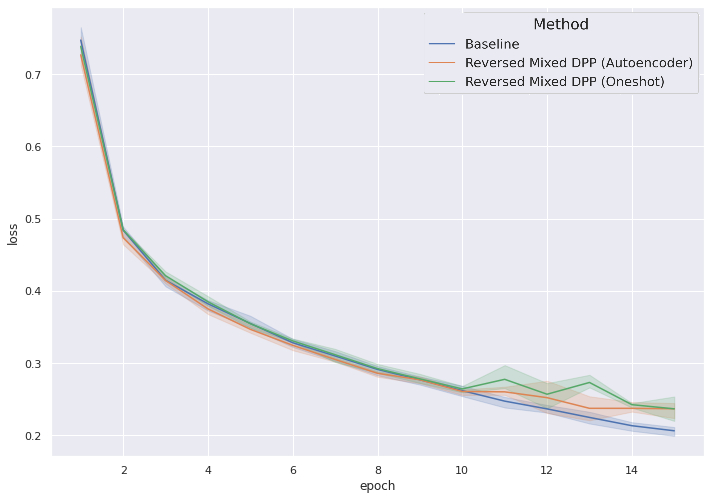
\includegraphics[width=8cm]{img/tesis/resultados/loss_nd_reversed_mixed.jpg}
    \caption{Resultados Reversed Mixed DPP en dataset clasificación multiclase (5 iteraciones), M = 400.}
    \label{fig:nd_reversed_mixed_dpp}
\end{figure}

Por otro lado, los resultados de \textit{Reversed Mixed DPP} en la Figura \ref{fig:nd_reversed_mixed_dpp} tampoco fueron exitosos, pues, al entrenar con menos ejemplos en las últimas épocas donde la reducción de la función de \textit{loss} es de menor magnitud en comparación al inicio, resultó en una pérdida de \textit{performance} general. Se analiza la posibilidad de trabajo a futuro con respecto a una metodología que cambie la estrategia de sampleo de \textit{batches} cuando la disminución de \textit{loss} sea despreciable. 

\begin{images}[\label{fig:time_nd_metric}]{\centering Tiempo de Entrenamiento Oneshot y Autoencoder en dataset clasificación multiclase.}
    \addimage{img/tesis/resultados/time_nd_oneshot.png}{width=7cm}{Tiempo Entrenamiento Oneshot}
    \addimage{img/tesis/resultados/time_nd_autoencoder.png}{width=7cm}{Tiempo Entrenamiento Autoencoder}
\end{images}


Los resultados que hemos obtenido hasta ahora son dependientes del aprendizaje de la métrica mediante \textit{Oneshot} o aprendiendo una representación de baja dimensionalidad mediante un \textit{Autoencoder}. El tiempo de entrenamiento se reporta en \ref{fig:time_nd_metric}. Si bien este debería ser sumado al tiempo de entrenamiento en \ref{fig:nd_mixed_dpp} (c), para el caso de la métrica con \textit{Oneshot} (a) el resultado no cambia pero para el \textit{Autoencoder} (b) el resultado resulta equivalente a la metodología \textit{baseline}.

\vspace{0.2cm}

Este detalle puede ser tratado de múltiples formas, desde el uso de \textit{Autoencoders} o redes \textit{Oneshot} menos profundas (con el fin de reducir el tiempo de entrenamiento), la búsqueda de métricas que no dependan del entrenamiento de una red (como las distancias de \textit{Minkowski} discutidas en \ref{section:minkowski}) o la que se propone en el Algoritmo \ref{alg:alg7} que se denomina DPP NET cuyo objetivo es el de entrenar en paralelo la red encargada de obtener la representación mientras se resuelve el problema de clasificación utilizando un sampleo con DPP. La siguiente sección detalla los resultados obtenidos por esta red. 


\section{DPP NET}

Las propuestas de métricas de distancia que hemos desarrollado durante la tesis incluyen el entrenamiento de una red \textit{Autoencoder} o \textit{Oneshot} que podría eventualmente tomar más tiempo que el entrenamiento de la red encarga de clasificar. Si bien esto depende del problema en específico y la profundidad con la que se trabaje cada red, se hace necesario la búsqueda de alternativas con las que realizar este proceso. 

\vspace{0.2cm}

La propuesta en este escenario es la de entrenar en paralelo la red encargada de definir la métrica y la red encargada de la clasificación, en este ejemplo, entrenar un \textit{Autoencoder} encargado de obtener la representación de baja dimensionalidad para utilizarla en el DPP y a su vez, utilizarla como \textit{input} para la red encargada de la clasificación. Por otro lado, con el fin de hacer la red lo más comparable posible a un \textit{baseline}, se hace uso de \textit{Fast DPP} para la reducción en los tiempos de entrenamiento.

\begin{images}[\label{fig:nd_dpp_net}]{\centering Resultados DPP NET en dataset clasificación multiclase (5 iteraciones), M = 400.}
    \addimage{img/tesis/resultados/loss_nd_dpp_net.png}{width=7cm}{Train loss según época}
    \addimage{img/tesis/resultados/time_nd_dpp_net.png}{width=7cm}{Train loss según tiempo}
\end{images}

La Figura \ref{fig:nd_dpp_net} muestra los resultados obtenidos por la metodología DPP NET que hace uso de la reducción de tiempo de entrenamiento gracias a \textit{Fast DPP}. Como se puede apreciar, el resultado alcanzado es desfavorable para nuestra metodología pues se ve ampliamente superada por el \textit{baseline}. 

\vspace{0.2cm}

Un resultado interesante del entrenamiento se puede ver alrededor de la época 4, pues el \textit{CNN loss} comienza a disminuir de manera considerable en la metodología DPP NET. Lo anterior puede ser explicado por el entrenamiento del \textit{Autoencoder} cuya mejora (aunque pequeña) en \textit{performance} hace que la métrica de distancia consumida por el DPP sea más precisa. 

\begin{images}[\label{fig:nd_autoencoder_dpp_net}]{\centering Entrenamiento Autoencoder en DPP NET.}
    \addimage{img/tesis/resultados/loss_nd_autoencoder_dpp_net.png}{width=7cm}{Train loss según época}
    \addimage{img/tesis/resultados/time_nd_autoencoder_dpp_net.png}{width=7cm}{Train loss según tiempo}
\end{images}

De los parámetros del experimento descritos en \ref{table:dppnet_parameters}, uno de gran importancia en el entrenamiento de la red DPP NET es el $\alpha = 1/3$ que controla en qué proporción impacta en \textit{loss} general el error de cada red por separado (como lo describe la arquitectura \ref{fig:dpp_net}). En este caso, notar que en la Figura \ref{fig:nd_autoencoder_dpp_net} (b) alcanza un \textit{loss} de 0.36 a los 280 segundos aproximadamente, a diferencia del entrenamiento del \textit{Autoencoder} en \ref{fig:time_nd_metric} (b) que alcanza un 0.32 en 100 segundos aproximadamente. En otras palabras, en DPP NET el \textit{Autoencoder} aún no alcanzaba un \textit{performance} aceptable que permitiera el uso correcto de un DPP mediante el aprendizaje de la métrica.

\vspace{0.2cm}

Distintas estrategias pueden tomarse a partir de este punto, como controlar el valor de $\alpha$ de manera dinámica con el fin de priorizar el entrenamiento del \textit{Autoencoder} en un principio y luego que este ya tenga un rendimiento aceptable, priorizar el entrenamiento de la red que clasifica (por ejemplo, desconectando o disminuyendo el entrenamiento del \textit{Autoencoder}). También se puede trabajar en la creación de una nueva estructura que utilice un aprendizaje de métrica como \textit{Oneshot learning} que podría disminuir los tiempos de entrenamiento. Finalmente, hacer uso de un esquema mixto de entrenamiento similar al propuesto en \textit{Mixed DPP} también podría resultar en mejoras sustanciales al modelo. 


